\subsection{Coefficient of Performance: V1}
The coefficient of performance is a measure of the useful energy transferred to the water in the tank per the system's supplied work. In other words, how much thermal energy can one get from 100 W input power, for example. The data obtained from this section are from EMCB use cases. There were different equations obtained from different resources \cite{LeightonClarke}, \cite{Shapiro2016FieldPO}, and \cite{Hudon}. All the aforementioned equations result in the following:
\begin{equation}\label{eq:cop}
    COP = \frac{Q}{E_{input}} = \frac{m \cdot C_{p} \cdot \Delta T}{E_{input}}
\end{equation}
Where:
\begin{itemize}
    \item m is the mass of the water in the tank in Pounds (lbm)
    \item $C_{p}$ is the specific heat of water ($\frac{Btu}{lbm \cdot \circ F}$)
    \item $\Delta T$ is the difference between the ambient temperature and the tank temperature in F.
    \item $E_{input}$ is the electrical power input in Watts. This includes the compressor and the heating element.
\end{itemize}

Equation \ref{eq:cop} is applied to the morning shower in the EMCB studies. The morning shower is a 20 gallon water draw. The change in the water temperature during the heating process is linear. Therefore, a cumulative sum of the input power and then the average were calculated which resulted in 1680 W. Here's a list of the numerical value in equation \ref{eq:cop}:
\begin{itemize}
    \item $E_{input}$ = 1680 W.
    \item m = 50 gallon $\times$ 8.34 = 417 lbm.
    \item C$_{p}$ = 1.001 $\frac{Btu}{lbm \cdot ^{\circ}F}$.
    \item $T_{ambient}$ = 75 $^{\circ}$F
\end{itemize}

For example, if the current temperature in the tank is 100 $^{\circ}F$, then the COP can be calculated as follows:

\begin{equation}
    COP = \frac{(417 [lbm] \times 1.001 \frac{Btu}{lbm \cdot F} \times (100 - 75) [F]) \times 0.293 }{1680 [W]}
    &=1.82
\end{equation}

\begin{figure}[htp!]
    \centering
    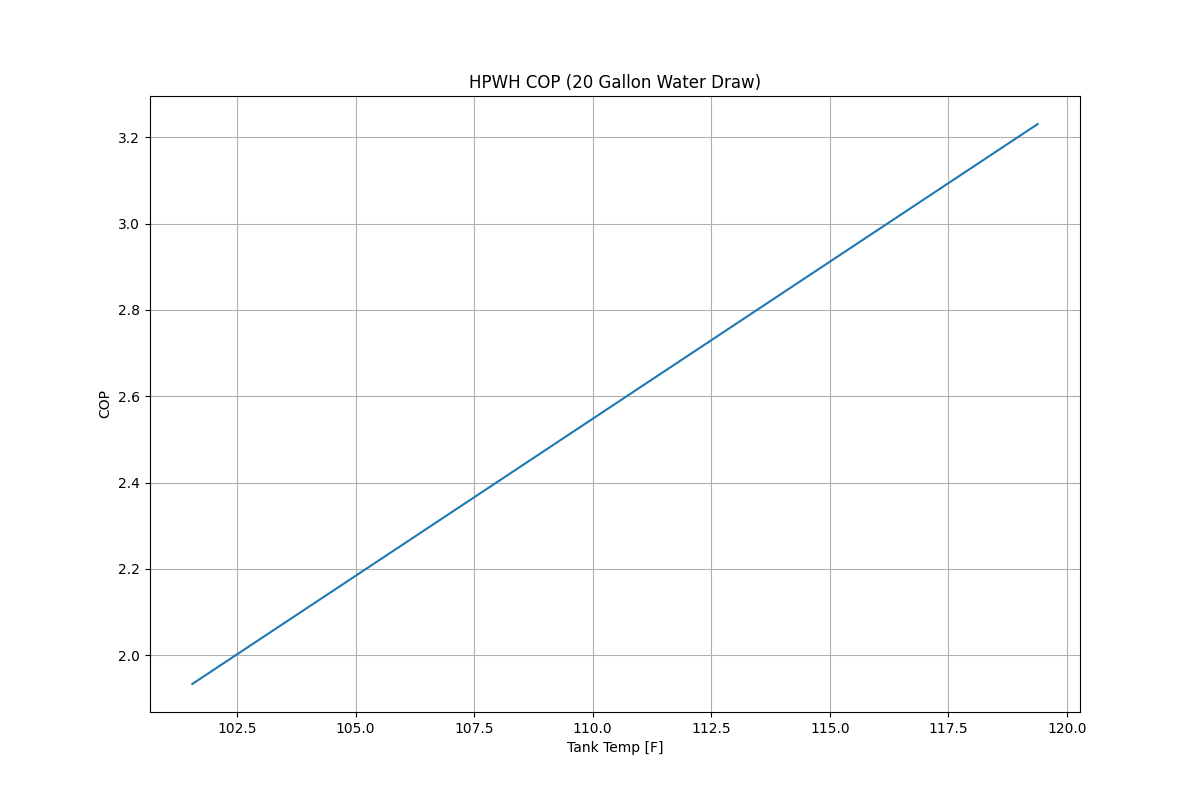
\includegraphics[width=1.1\columnwidth]{Pictures/cop_sim.png}
    \caption{HPWH COP: 20 Gallon Water Draw}
    \label{fig:cop}
\end{figure}
\newpage
\subsection{Coefficient of Performance: V2}
The equation used to calculate and plot the COP of the HPWH is as follows:

\begin{equation}
    COP = \frac{EnergyTake}{Watts}
\end{equation}
The HPWH was set to vacation mode for three days. After, the HPWH was switched to Hybrid mode. Here's the data when the HPWH switch ON.

\begin{longtable}{|l|l|l|}
\hline
time & EnergyTake & Watts  \\ \hline
\endhead
%
Mon Sep 20 12:17:12 2021 &               2775 &       4449.0300 \\ \hline
Mon Sep 20 12:18:12 2021 &               2775 &       4665.8100 \\ \hline
Mon Sep 20 12:19:13 2021 &               2625 &       4686.4500 \\ \hline
Mon Sep 20 12:20:14 2021 &               2550 &       4717.4200 \\ \hline
Mon Sep 20 12:21:14 2021 &               2250 &       4738.0600 \\ \hline
Mon Sep 20 12:22:15 2021 &               2175 &       4748.3900 \\ \hline
Mon Sep 20 12:23:15 2021 &               2025 &       4707.1000 \\ \hline
Mon Sep 20 12:24:16 2021 &               2025 &       4769.0300 \\ \hline
Mon Sep 20 12:25:17 2021 &               1875 &       4769.0300 \\ \hline
Mon Sep 20 12:26:17 2021 &               1800 &       4758.7100 \\ \hline
Mon Sep 20 12:27:18 2021 &               1725 &       4769.0300 \\ \hline
Mon Sep 20 12:28:18 2021 &               1725 &       4769.0300 \\ \hline
Mon Sep 20 12:29:19 2021 &               1650 &       4779.3500 \\ \hline
Mon Sep 20 12:30:19 2021 &               1575 &       4676.1300 \\ \hline
Mon Sep 20 12:31:20 2021 &               1575 &       4707.1000 \\ \hline
Mon Sep 20 12:32:21 2021 &               1425 &       4645.1600 \\ \hline
Mon Sep 20 12:33:21 2021 &               1425 &       4696.7700 \\ \hline
Mon Sep 20 12:34:22 2021 &               1275 &       4696.7700 \\ \hline
Mon Sep 20 12:35:22 2021 &               1200 &       4686.4500 \\ \hline
Mon Sep 20 12:36:23 2021 &               1050 &        392.2580 \\ \hline
Mon Sep 20 12:37:24 2021 &               1050 &        402.5810 \\ \hline
Mon Sep 20 12:38:24 2021 &               1050 &        402.5810 \\ \hline
Mon Sep 20 12:39:25 2021 &                975 &        402.5810 \\ \hline
Mon Sep 20 12:40:25 2021 &                975 &        402.5810 \\ \hline
Mon Sep 20 12:41:26 2021 &                975 &        402.5810 \\ \hline
Mon Sep 20 12:42:27 2021 &                975 &        402.5810 \\ \hline
Mon Sep 20 12:43:27 2021 &                975 &        402.5810 \\ \hline
Mon Sep 20 12:44:28 2021 &                975 &        402.5810 \\ \hline
Mon Sep 20 12:45:28 2021 &                975 &        402.5810 \\ \hline
Mon Sep 20 12:46:29 2021 &                975 &        412.9030 \\ \hline
Mon Sep 20 12:47:29 2021 &                975 &        402.5810 \\ \hline
Mon Sep 20 12:48:30 2021 &                975 &        402.5810 \\ \hline
Mon Sep 20 12:49:31 2021 &                975 &        402.5810 \\ \hline
Mon Sep 20 12:50:31 2021 &                900 &        402.5810 \\ \hline
Mon Sep 20 12:51:32 2021 &                900 &        412.9030 \\ \hline
Mon Sep 20 12:52:32 2021 &                825 &        412.9030 \\ \hline
Mon Sep 20 12:53:33 2021 &                825 &        402.5810 \\ \hline
Mon Sep 20 12:54:34 2021 &                825 &        412.9030 \\ \hline
Mon Sep 20 12:55:34 2021 &                825 &        412.9030 \\ \hline
Mon Sep 20 12:56:35 2021 &                825 &        412.9030 \\ \hline
Mon Sep 20 12:57:35 2021 &                825 &        412.9030 \\ \hline
Mon Sep 20 12:58:36 2021 &                825 &        412.9030 \\ \hline
Mon Sep 20 12:59:36 2021 &                825 &        412.9030 \\ \hline
Mon Sep 20 13:00:37 2021 &                750 &        412.9030 \\ \hline
Mon Sep 20 13:01:38 2021 &                750 &        412.9030 \\ \hline
Mon Sep 20 13:02:38 2021 &                750 &        412.9030 \\ \hline
Mon Sep 20 13:03:39 2021 &                750 &        412.9030 \\ \hline
Mon Sep 20 13:04:39 2021 &                600 &        412.9030 \\ \hline
Mon Sep 20 13:05:40 2021 &                600 &        423.2260 \\ \hline
Mon Sep 20 13:06:41 2021 &                600 &        423.2260 \\ \hline
Mon Sep 20 13:07:41 2021 &                600 &        423.2260 \\ \hline
Mon Sep 20 13:08:42 2021 &                600 &        423.2260 \\ \hline
Mon Sep 20 13:09:42 2021 &                600 &        423.2260 \\ \hline
Mon Sep 20 13:10:43 2021 &                600 &        423.2260 \\ \hline
Mon Sep 20 13:11:43 2021 &                600 &        423.2260 \\ \hline
Mon Sep 20 13:12:44 2021 &                600 &        423.2260 \\ \hline
Mon Sep 20 13:13:45 2021 &                600 &        423.2260 \\ \hline
Mon Sep 20 13:14:45 2021 &                525 &        423.2260 \\ \hline
Mon Sep 20 13:15:46 2021 &                525 &        423.2260 \\ \hline
Mon Sep 20 13:16:46 2021 &                525 &        423.2260 \\ \hline
Mon Sep 20 13:17:47 2021 &                525 &        423.2260 \\ \hline
Mon Sep 20 13:18:48 2021 &                525 &        433.5480 \\ \hline
Mon Sep 20 13:19:48 2021 &                525 &        433.5480 \\ \hline
Mon Sep 20 13:20:49 2021 &                525 &        433.5480 \\ \hline
Mon Sep 20 13:21:49 2021 &                525 &        433.5480 \\ \hline
Mon Sep 20 13:22:50 2021 &                450 &        433.5480 \\ \hline
Mon Sep 20 13:23:51 2021 &                450 &        433.5480 \\ \hline
Mon Sep 20 13:24:51 2021 &                375 &        433.5480 \\ \hline
Mon Sep 20 13:25:52 2021 &                375 &        433.5480 \\ \hline
Mon Sep 20 13:26:52 2021 &                375 &        433.5480 \\ \hline
Mon Sep 20 13:27:53 2021 &                375 &        433.5480 \\ \hline
Mon Sep 20 13:28:53 2021 &                375 &        433.5480 \\ \hline
Mon Sep 20 13:29:54 2021 &                225 &        433.5480 \\ \hline
Mon Sep 20 13:30:55 2021 &                225 &        433.5480 \\ \hline
Mon Sep 20 13:31:55 2021 &                225 &        433.5480 \\ \hline
Mon Sep 20 13:32:56 2021 &                225 &        433.5480 \\ \hline
Mon Sep 20 13:33:56 2021 &                225 &        433.5480 \\ \hline
Mon Sep 20 13:34:57 2021 &                225 &        433.5480 \\ \hline
Mon Sep 20 13:35:58 2021 &                225 &        443.8710 \\ \hline
Mon Sep 20 13:36:58 2021 &                225 &        443.8710 \\ \hline
Mon Sep 20 13:37:59 2021 &                225 &        443.8710 \\ \hline
Mon Sep 20 13:38:59 2021 &                 75 &        443.8710 \\ \hline
Mon Sep 20 13:40:00 2021 &                 75 &        443.8710 \\ \hline
Mon Sep 20 13:41:01 2021 &                 75 &        433.5480 \\ \hline
Mon Sep 20 13:42:01 2021 &                 75 &        433.5480 \\ \hline
Mon Sep 20 13:43:02 2021 &                 75 &        433.5480 \\ \hline
Mon Sep 20 13:44:02 2021 &                 75 &        443.8710 \\ \hline
Mon Sep 20 13:45:03 2021 &                 75 &        443.8710 \\ \hline
Mon Sep 20 13:46:03 2021 &                  0 &        443.8710 \\ \hline
Mon Sep 20 13:47:04 2021 &                  0 &        443.8710 \\ \hline
Mon Sep 20 13:48:05 2021 &                  0 &        443.8710 \\ \hline
Mon Sep 20 13:49:05 2021 &                  0 &        454.1940 \\ \hline
Mon Sep 20 13:50:06 2021 &                  0 &        443.8710 \\ \hline
Mon Sep 20 13:51:06 2021 &                  0 &        454.1940 \\ \hline
Mon Sep 20 13:52:07 2021 &                  0 &        454.1940 \\ \hline
Mon Sep 20 13:53:07 2021 &                  0 &        454.1940 \\ \hline
Mon Sep 20 13:54:08 2021 &                  0 &        443.8710 \\ \hline
Mon Sep 20 13:55:08 2021 &                  0 &        454.1940 \\ \hline
Mon Sep 20 13:56:09 2021 &                  0 &        454.1940 \\ \hline
Mon Sep 20 13:57:09 2021 &                  0 &        454.1940 \\ \hline
Mon Sep 20 13:58:10 2021 &                  0 &        454.1940 \\ \hline
Mon Sep 20 13:59:11 2021 &                  0 &        454.1940 \\ \hline
Mon Sep 20 14:00:11 2021 &                  0 &        454.1940 \\ \hline
Mon Sep 20 14:01:12 2021 &                  0 &        454.1940 \\ \hline
Mon Sep 20 14:02:12 2021 &                  0 &        454.1940 \\ \hline
Mon Sep 20 14:03:13 2021 &                  0 &        454.1940 \\ \hline
Mon Sep 20 14:04:13 2021 &                  0 &        454.1940 \\ \hline
Mon Sep 20 14:05:14 2021 &                  0 &        464.5160 \\ \hline
Mon Sep 20 14:06:15 2021 &                  0 &        454.1940 \\ \hline
Mon Sep 20 14:07:15 2021 &                  0 &        454.1940 \\ \hline
Mon Sep 20 14:08:16 2021 &                  0 &        454.1940 \\ \hline
Mon Sep 20 14:09:16 2021 &                  0 &        454.1940 \\ \hline
Mon Sep 20 14:10:17 2021 &                  0 &        454.1940 \\ \hline
Mon Sep 20 14:11:17 2021 &                  0 &         41.2903 \\ \hline
Mon Sep 20 14:12:18 2021 &                  0 &         30.9677 \\ \hline
Mon Sep 20 14:13:19 2021 &                  0 &         41.2903 \\ \hline
Mon Sep 20 14:14:19 2021 &                  0 &         41.2903 \\ \hline
Mon Sep 20 15:20:57 2021 &                  0 &         10.3226 \\ \hline

\end{longtable}

The HPWH was ON for 81 minutes to heat the water up to the setpoints, 120 $^{\circ}F$. Therefore, the values of watts consumed was converted to Watts-hour as follows:
\begin{equation}
    Wh = Watts \times \frac{x-1}{60}
\end{equation}
Where x is the duration of the heating process.

The following figures show the COP VS:
\begin{itemize}
    \item time
    \item EnergyTake
    \item Line fit
\end{itemize}
\textbf{The average COP is 3.2}

\begin{figure}[htp!]
    \centering
    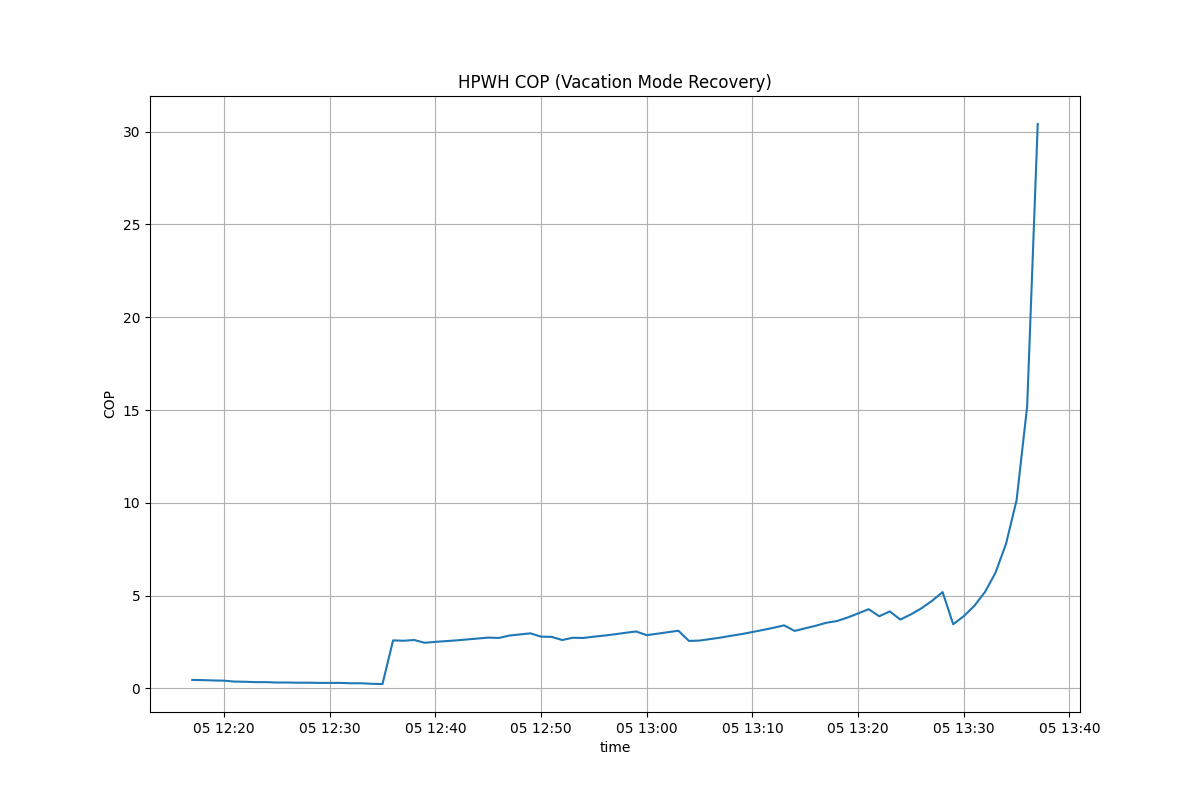
\includegraphics[width=1.1\columnwidth]{Pictures/cop_vs_time.png}
    \caption{HPWH COP vs Time: Vacation Mode Recovery}
    \label{fig:copvstime}
\end{figure}

\begin{figure}[htp!]
    \centering
    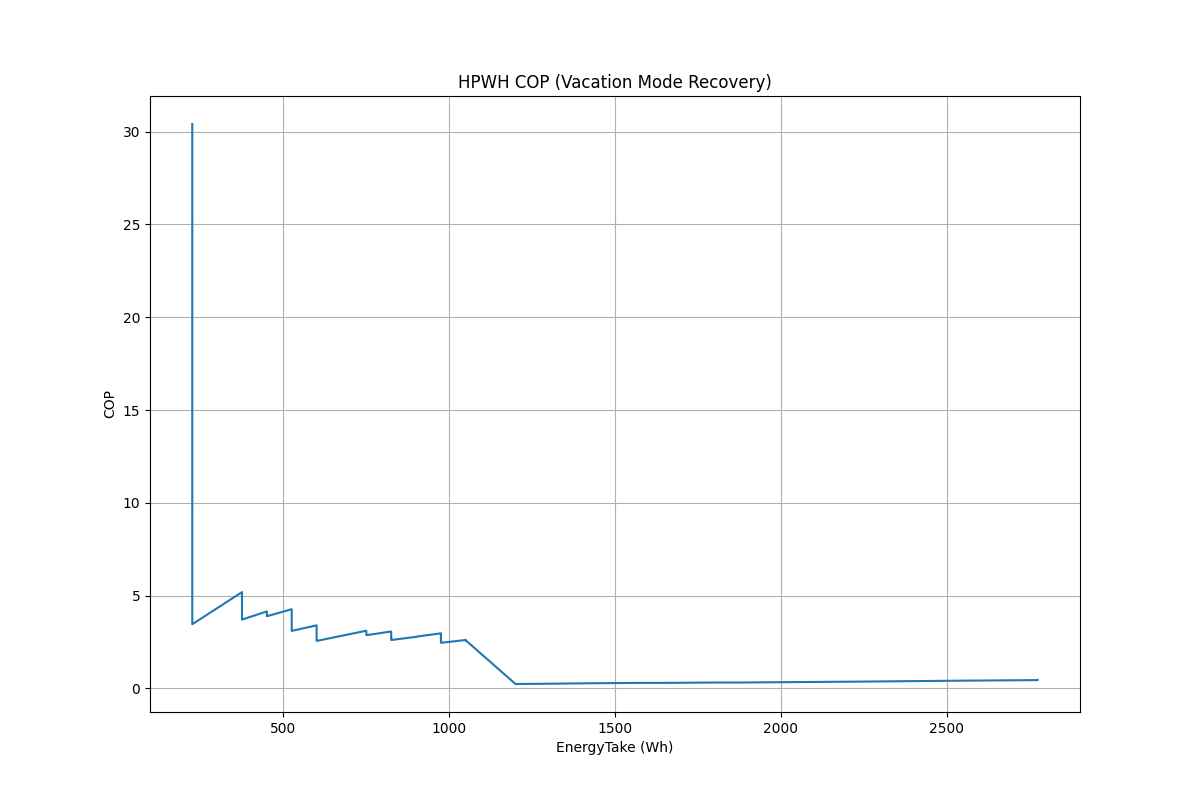
\includegraphics[width=1.1\columnwidth]{Pictures/cop_vs_EnergyTake.png}
    \caption{HPWH COP vs EnergyTake: Vacation Mode Recovery}
    \label{fig:copvsenergytake}
\end{figure}
\newpage

\subsection{this should work in a good position}
